%%
%% Copyright 2007, 2008, 2009 Elsevier Ltd
%%
%% This file is part of the 'Elsarticle Bundle'.
%% ---------------------------------------------

%% Please read the file, ``Addtional_AuthorInstruction_LaTeX.pdf'', for choosing the following options. 
%% Please choose only one of the two following options. Note that the option \final, which is also provided below, must not be submitted.
%\def\preprint{1}		% Use for submitted manuscript
\def\wordcount {1}		% Use for word count

%% The following option provides the final print version. This is only for personal use. Don't use this for submission.
%\def\final {1}			

%% Please do not modify the following nine lines
\ifdefined\preprint
  \documentclass[preprint,review,12pt]{elsarticle}
\fi
\ifdefined\wordcount
  \documentclass[final,3p,times,twocolumn]{elsarticle}
\fi
\ifdefined\final
  \documentclass[final,3p,times,twocolumn]{elsarticle}
\fi

%% Graphics packages for PostScript figures 
\usepackage{amsfonts}
\usepackage{amsmath}
\usepackage{amsthm}
\usepackage{amssymb}
\usepackage{breqn}
\usepackage{chemformula}
\usepackage{float}
\usepackage{footnote}
%\usepackage[hang,flushmargin,bottom]{footmisc} % footnote format
\usepackage{graphicx}
\usepackage[utf8]{inputenc}
\usepackage{latexsym}
\usepackage{mathptmx}
\usepackage{multirow}
\usepackage{siunitx}
\usepackage{subfigure}
\usepackage{threeparttable}
\usepackage{textgreek}
\usepackage{xcolor}

\biboptions{sort&compress}

\journal{Proceedings of the Combustion Institute}

\begin{document}

\begin{frontmatter}

\title{Mixture Fraction Analysis of Combustion Products in Medium-Scale Pool Fires}

\author{Ryan Falkenstein-Smith\corref{cor1}}
\ead{ryan.falkenstein-smith@nist.gov}

\author{Kunhyuk Sung}
\author{Anthony Hamins}

\address{National Institute of Standards and Technology, 100 Bureau Dr., Gaithersburg, MD 20899, United States of America}
\cortext[cor1]{Corresponding author: Ryan Falkenstein-Smith}

\begin{abstract}
A mixture fraction analysis is performed to investigate the characteristics of time-averaged gaseous species measurements made along the centerline of medium-scale pool fires steadily burning in a quiescent environment. A series of fire experiments are conducted using 30~cm diameter liquid and 38~cm diameter gaseous pool burners. All gaseous species measurements are obtained using a Gas Chromatograph with a mass selectivity detector for gas samples extracted at various heights within the fire. Soot mass fractions are simultaneously measured during gas sampling. For all fuels, the results show that the local composition plotted as a function of mixture fraction collapses the experimental data into a few coherent lines that nearly match the idealized reactions. Differences between the theoretical and experimental data are attributed to the presence of carbon monoxide soot and other intermediate carbon-containing species.
\end{abstract}

\begin{keyword}

Mixture fraction \sep Pool fires \sep Carbon-to-Hydrogen Ratio \sep Combustion Products \sep Chemical Composition

\end{keyword}

\end{frontmatter}


%% Please do not modify the following three lines
\ifdefined \wordcount
\clearpage
\fi

\section{Introduction}
\label{Introduction}
Computational fluid dynamics (CFD) models are an important component of performance-based design in fire protection engineering. A requirement of their acceptance in the design process is that these models be verified and validated, the latter of which involves comparison with experimental measurements. The primary objective of this work is to provide data for use in fire model validation. 

The mixture fraction-based combustion has been widely used to characterize the combustion chemistry of different fires~\cite{Bilger1977,Peters1984,Floyd2001,Hamins1987,Sivathanu1990}, which is essential when improving the accuracy of fire model predictions. A mixture fraction-based combustion model assumes that the combustion is mixing-controlled, and the reaction between fuel and oxygen is taking place on an infinitely thin flame sheet. This assumption is ideal for well-ventilated conditions such as a pool fire. 

In a pool fire, the fuel surface is isothermal, flat and horizontal, providing a well-defined boundary condition for modeling. Fuel and product species concentrations and temperatures have a significant influence on the heat feedback to the fuel surface, which directly affects the burning rate. A zone of particular interest is the fuel rich-core between the flame and the pool surface, where gaseous species can absorb energy that would otherwise have been transferred to the fuel surface. Few studies in the literature have reported local chemical species measurements within the flame envelope.

In this study, a mixture fraction analysis is performed to investigate the characterize the spatial distribution of the principal chemical species in moderate-scale pool fires steadily burning in a well-ventilated, quiescent environment. A series of fire experiments was conducted using a 30~cm diameter liquid and 38~cm diameter gaseous pool burner. Gaseous species and soot measurements were made at various heights within the fire. Four kinds of fuels are considered, namely, methanol, ethanol, acetone, and methane. Through the analysis of the species composition at various locations within the fire, this study attempts to provide insight into the combustion chemistry of pool fires. 


\section{Description of Experiments}
\label{sec:Experiments}

\subsection{Pool Burner Setup}
\label{ssec:Pool_Burner_Setup}
All experiments are conducted under a canopy hood surrounded by an enclosure 2.5~m on a side made of a double layer wire-mesh screen (5 mesh/cm) to reduce the impact of room ventilation. All measurements are made once the mass burning rate reaches a steady-state, achieved approximately 10~min and 2~min after ignition for the liquid and gaseous fuels, respectively.

Liquid fuels are burned in a circular, stainless-steel pan, made from cold-rolled steel, with an outer diameter of 30~cm, a depth of 15~cm, and a wall thickness of 1.6~mm. The lip of the liquid burner is positioned 30~cm above the floor. The liquid burner has an overflow basin, which extends 3~cm beyond the burner wall. Fuel to the liquid burner is gravity fed from a reservoir positioned on a mass load cell located outside the enclosure and is manually controlled by adjusting the fuel flow using a needle valve. The fuel surface is maintained 10~mm below the burner rim to match previous experimental conditions \cite{Fisher1987,Hamins2016,Kim2019,Weckman1996}. Gaseous fuels are burned using a 38~cm diameter burner. Fuel to the gaseous burner is controlled via a mass flow controller located outside of the enclosure. The bottoms of both burners are maintained at a constant temperature by flowing water ($20 \; ^\circ \hbox{C} \pm 3 \; ^\circ \hbox{C}$). Further descriptions of the liquid and gaseous burners are found in Refs.~\cite{Hamins2016,Hamins1994,Hamins1991,Hamins1996,Lock2008,Hamins1996a}.

The mean flame height, $L_{\rm{f}}$, is estimated from 3600~frames of high-resolution video of the experiments using MATLAB’s Image Processing Toolbox\footnote{\label{fn:product} Certain commercial products are identified in this report to specify adequately the equipment used. Such identification does not imply a recommendation by the National Institute of Standards and Technology, nor does it imply that this equipment is the best available for the purpose.}. Imported color images are decomposed into binary (i.e., black and white) images using a pre-set threshold level. The flame height for a single frame is defined as the distance between the pool surface and flame tip. All measurements are repeated, then averaged to provide the mean flame height.

\subsection{Measuring the Volume Fraction of Gaseous Species}
\label{ssec:Gas_Species_Setup}

Gaseous species measurements are made using an Agilent 5977E Series Gas Chromatograph with a mass selectivity detector (GC/MSD) fitted with a thermal conductivity detector. Figure~\ref{fig:Experimental_Setup} displays the flow diagram for gas sampling. The gases are extracted by a vacuum pump located downstream of the GC/MSD. Gas samples are collected using a quenching probe, which is composed of two concentric, stainless-steel tubes with outer annular coolant flow and inner, extracted sample flow. The inner and outer tube diameters are \SI{8}{mm} and \SI{16}{mm}, respectively. Water at approximately \SI{90}{\degree C} flows through the sampling probe during sampling. The remainder of the sampling line leading into the GC/MSD is heated with electrical, heating tape to approximately \SI{140}{\degree C} to prevent condensation of water and liquid fuels within the line.

\begin{figure*}
	\centering
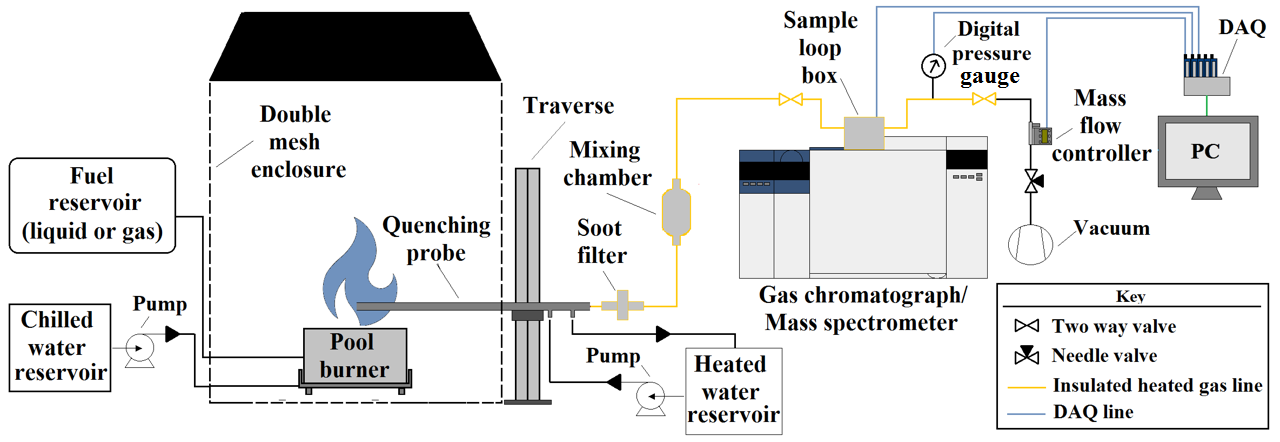
\includegraphics[width=14.4 cm,keepaspectratio]{Experimental_Setup.png}
	\caption[A schematic of the gas sampling procedure]{A schematic of the extraction sampling and analysis system.}
	\label{fig:Experimental_Setup}
\end{figure*}
Depending on the probe location within the fire, the sampling period varies from \SI{12}{min} to \SI{25}{min}, ensuring a sufficient mass of gaseous sample and soot is collected. The flow is controlled using a mass flow controller (Alicat Scientific MC-Series) located in front of the vacuum pump within the sampling line. During the gas sampling procedure, the volumetric flow is approximately 200~mL/min and recorded at \SI{2}{\hertz}. All measurements using the GC/MSD are repeated at least twice at each location along the centerline of the pool fire. Gaseous species concentration measurements made at the same location are averaged. The mean mass fraction, $\bar{Y}_{i}$, of a given species $i$ is calculated from the measured volume fraction, $\bar{X}_{i}$, using the following expression:
\begin{equation}\label{eq:mass_fraction}
	\bar{Y}_{i}=\frac{\bar{X}_{i} \, {\textrm{W}_{i}}}{\sum{\bar{X}_{i} \, {\textrm{W}_{i}}}}
\end{equation}
where ${{\textrm{W}_{i}}}$ is the molecular weight of a given species.

\subsection{Centerline Temperature Measurements}
\label{ssec:Temperature_Measurements}
Time-averaged temperature measurements were made along the centerline profiles of the pool fires at the same gas sampling locations. An S-type (Pt 10\% Rh/Pt), bare-wire, fine diameter thermocouple (OMEGA P10R-001) with a wire diameter of approximately 50~$\mu$m and a bead diameter of approximately 150~$\mu$m was used. Temperature measurements are sampled at \SI{250}{Hz} for \SI{2}{min}, or approximately 300~pulsing cycles \cite{Wang2019}. The thermal inertia and radiative heat loss associated with the thermocouple were corrected following the method of Shaddix~\cite{Shaddix1999}. 

\subsection{Determining Soot Mass Fraction}
\label{ssec:Soot_Setup}
Soot mass fraction, $Y_{\rm s}$, is measured using a well established gravimetric technique~\cite{Choi1995}. Soot is filtered out of the gas stream using a stainless steel particulate filter holder (PALL 2220). Before an experiment, a desiccated \SI{47}{mm} polytetrafluoroethylene (PTFE) filter is weighed and placed into its holder. The filter holder is positioned within the gas sampling line behind the quenching probe and heated with tape to approximately \SI{140}{\degree C} to prevent condensation of water and liquid fuels on the filter. After sampling, the filter is removed and dried in a desiccator. After drying for 48~h, the filter’s final weight is measured. Approximately \SI{1}{mg} of soot is collected during the sampling period. The mass of the PTFE filter and cleaning patches are measured three times before and after each test. After most experiments, soot deposits are observed on the inner walls of the quenching probe. Dedicated gun cleaning patches (Hoppe's 9 1203S) are used to clean the inside of the quenching probe with no cleaning solvent. At least two patches are used to collect soot on the inside of the probe. A petri dish is placed below one end of the probe to catch dislodged soot and patches. Soot collection on the inside of the probe concludes once an applied patch is observed to have no soot. Patches are weighed immediately before and 48~h after cleaning the inside of the probe.

The soot mass fraction, $Y_{\rm s}$, is computed from the mass of the soot collected from the PTFE filter and gun cleaning patches, $m_{\rm s}$, the ratio of the mass flow controller's temperature reading, $T_{\infty}$, to the effective temperature of the gas obtained from the thermocouple measurements, $T_{\rm g}$, the total mass of gas sampled, $m_{\rm tot}$, based on the mass flow controller readings:
\begin{equation}\label{eq:overall_soot_mass_frac}
Y_{\rm s}= \frac{m_{\rm s} \, V_{s}}{\dot{V} \, \Delta t \, m_{\rm tot}}\frac{T_{\rm \infty}}{T_{\rm g}}
\end{equation}
where the total mass of gas sampled is represented by the product of the average volumetric flow rate measured by the mass flow controller, $\dot{V}$, the gas sampling time, $\Delta t$ and the total mass detected from the GC/MSD, $m_{\rm tot}$ over the injected sample volume, $V_{\rm s}$.
\subsection{Mixture Fraction Calculation}
\label{ssec:Mixture_Fraction_Calculation}
The mixture fraction, $Z$, is defined as the mass fraction of the gases containing carbon, in addition to soot, that originate in the fuel stream. It can be expressed as follows:
\begin{equation}\label{eq:Mixture_Fraction}
Z = \bar{Y}_{\rm F} + \frac{W_{\rm F}}{\rm x} \sum_{i\ne{\rm F}} \frac{\bar{Y}_i}{W_{i}}
\end{equation}
where $\bar{Y}_{\rm F}$, ${W_{\rm F}}$, and $\rm x$ are the mass fraction, molecular weight, and number of carbon atoms in the fuel molecule, respectively. Assuming ideal (i.e. no CO or soot), infinitely-fast (fuel and oxygen from the air cannot co-exist) combustion, the mass fractions of all species can be expressed as piece-wise linear ``state relations'' according to the following reaction:
\begin{multline}\label{eq:Ideal_rxn}
{\rm C}_{\rm x}{\rm H}_{\rm y}{\rm O}_{\rm z}\\ +\eta(\rm x+\frac{\rm y}{4}-\frac{\rm z}{2})~({\rm O}_{2}+3.76~{\rm N}_{2}+0.0445~{\rm Ar}) \rightarrow \\ \max(0,1-\eta)~{\rm C}_{\rm x}{\rm H}_{\rm y}{\rm O}_{\rm z}+\max(0,1- \eta)~(\rm x+\frac{\rm y}{4}-\frac{\rm z}{2})~{\rm O}_{2} \\ +\eta(\rm x+\frac{\rm y}{4}-\frac{\rm z}{2})~(3.76~{\rm N}_{2}+0.0445~{\rm Ar})\\+ \min(1,\eta)~\rm x~{\rm CO}_{2}+\min(1,\eta)~\frac{\rm y}{2}~{\rm H}_{2}{\rm O}
\end{multline}
The parameter $\eta$ is the reciprocal of the local fuel equivalence ratio, $\phi$,
\begin{equation}\label{eq:Eta}
\phi=\frac{\rm (F/A)}{{\rm (F/A)}_{\rm st}}=\frac{1}{\eta}
\end{equation}
where $\rm F/A$ is the fuel-air mass ratio and the subscript $\rm st$ denotes the stoichiometric condition.The idealized mass fractions of the products are obtained from the right side of Eq.~\ref{eq:Ideal_rxn}.
\subsection{Uncertainty Analysis}
\label{ssec:Uncertainty Analysis}
An extensive uncertainty of all measurements made in this study is provided in Ref.~\cite{Falkenstein2019}. The uncertainties of all measurements are calculated assuming a 95\% confidence level. The uncertainty of the mixture fraction is a function of the uncertainties in the carbon carrying species:
\begin{equation}
\label{eq:mixture_frac_uncertainty}
{u_{\scriptscriptstyle Z}}^2={{u_{\scriptscriptstyle \bar{Y}_{\rm F}}}^2+{\left(\frac{W_{\rm F}}{\rm x}\right)}^2{\sum_{i\ne {\rm F}}{\left(\frac{u_{\scriptscriptstyle \bar{Y}_{i}}}{\textrm{W}_{i}} \right)}^2}}
\end{equation}
where $u_{\scriptscriptstyle Z}$ is the estimated uncertainty of the mixture fraction determined from combined expanded uncertainty of the mass fractions of all carbon carrying species. 

\section{Results}
\label{sec:Results}

\subsection{Flame Observations}
\label{ssec:Flame_Observations}
The methanol fire is purely blue, whereas the ethanol, acetone, and methane fires are more luminous and yellow. The measured time-averaged burning rates and calculated heat release rates are listed in Table~\ref{tab:Pool_Fire_Parameters_Table}. The heat release rates are calculated from the product of the mass burning flux and the heat of combustion. The methanol fire has the lowest average flame height, followed by the ethanol, then the methane, and then the acetone. The measured mean flame heights match Heskestad’s correlation~\cite{Heskestad1983} to within measurement uncertainty. The measured flame heights are also within the uncertainty bounds of measurements made by Kim~et~al.~\cite{Kim2019}.

\begin{table}[!t]
\caption[List of measurements and thermochemical properties of fuels]{List of measurements and thermochemical properties of fuels burning in a well-ventilated round pool fire}
\label{tab:Pool_Fire_Parameters_Table}
\footnotesize
 %\centering
\resizebox{\columnwidth}{!}{%
	\begin{tabular}{lcccc}
\hline
%\\[0.0005cm]
\textbf{Parameter (units)} &\textbf{Methanol}& \textbf{Ethanol}& \textbf{Acetone}&\textbf{Methane}\\
\hline
\\[0.01cm]
Diameter~(\si{m})						&	30				&	30				&	30				& 	38			\\
\\[0.01cm]
Mass Burning Flux~(\si{g/{m^2 s}})		        	&	12.4~$\pm$~1.1		&	13.9~$\pm$~0.8		&	17.6~$\pm$~2.7		&	6.4~$\pm$~0.1	\\
\\[0.01cm]
Heat Release Rate~(\si{kW})		            	&	17.4~$\pm$~1.4		&	26.3~$\pm$~1.5		&	35.5~$\pm$~5.4		&	34.5~$\pm$~0.5	\\
\\[0.01cm]						
Mean Flame Height~(\si{cm})			           &	36.4~$\pm$~16.0		&	61.1~$\pm$~28.2		&	91.5~$\pm$~34.6		&	64.5~$\pm$~31.1	\\
\\[0.01cm]
Carbon/Hydrogen Ratio				         	&	1/4				&	1/3				&	1/2				&	1/4			\\
\\[0.01cm]
\hline
\end{tabular}
}
\end{table}

\subsection{Comparison of Pool Fires from Different Fuels}
\label{ssec:Fuel_comp}

Figure~\ref{fig:Temp_Comparison} displays the time-averaged gas temperatures as a function of the normalized vertical spatial coordinate, $z^*$:
\begin{equation}\label{eq:Z_Star}
z^*=\frac{z}{D^*}  \quad ; \quad  D^* = \left(\frac{\dot{Q}}{c_{p}\rho_\infty T_\infty \sqrt{g}}\right)^{\frac{2}{5}}
\end{equation}
Here, $z$ is the vertical spatial coordinate, $\dot{Q}$ is the heat release rate, $g$ is the acceleration of gravity, and $c_p$ and $\rho_\infty$ are the specific heat and the density of air at room temperature, $T_\infty$. The maximum mean temperature for each fuel peaks at approximately $z^*=0.68~\pm~0.21$. Methanol has the highest mean temperature of 1316~K with ethanol and acetone exhibiting maximum mean temperatures of 1281~K and 1190~K, respectively.

\begin{figure}[h!]
	\centering
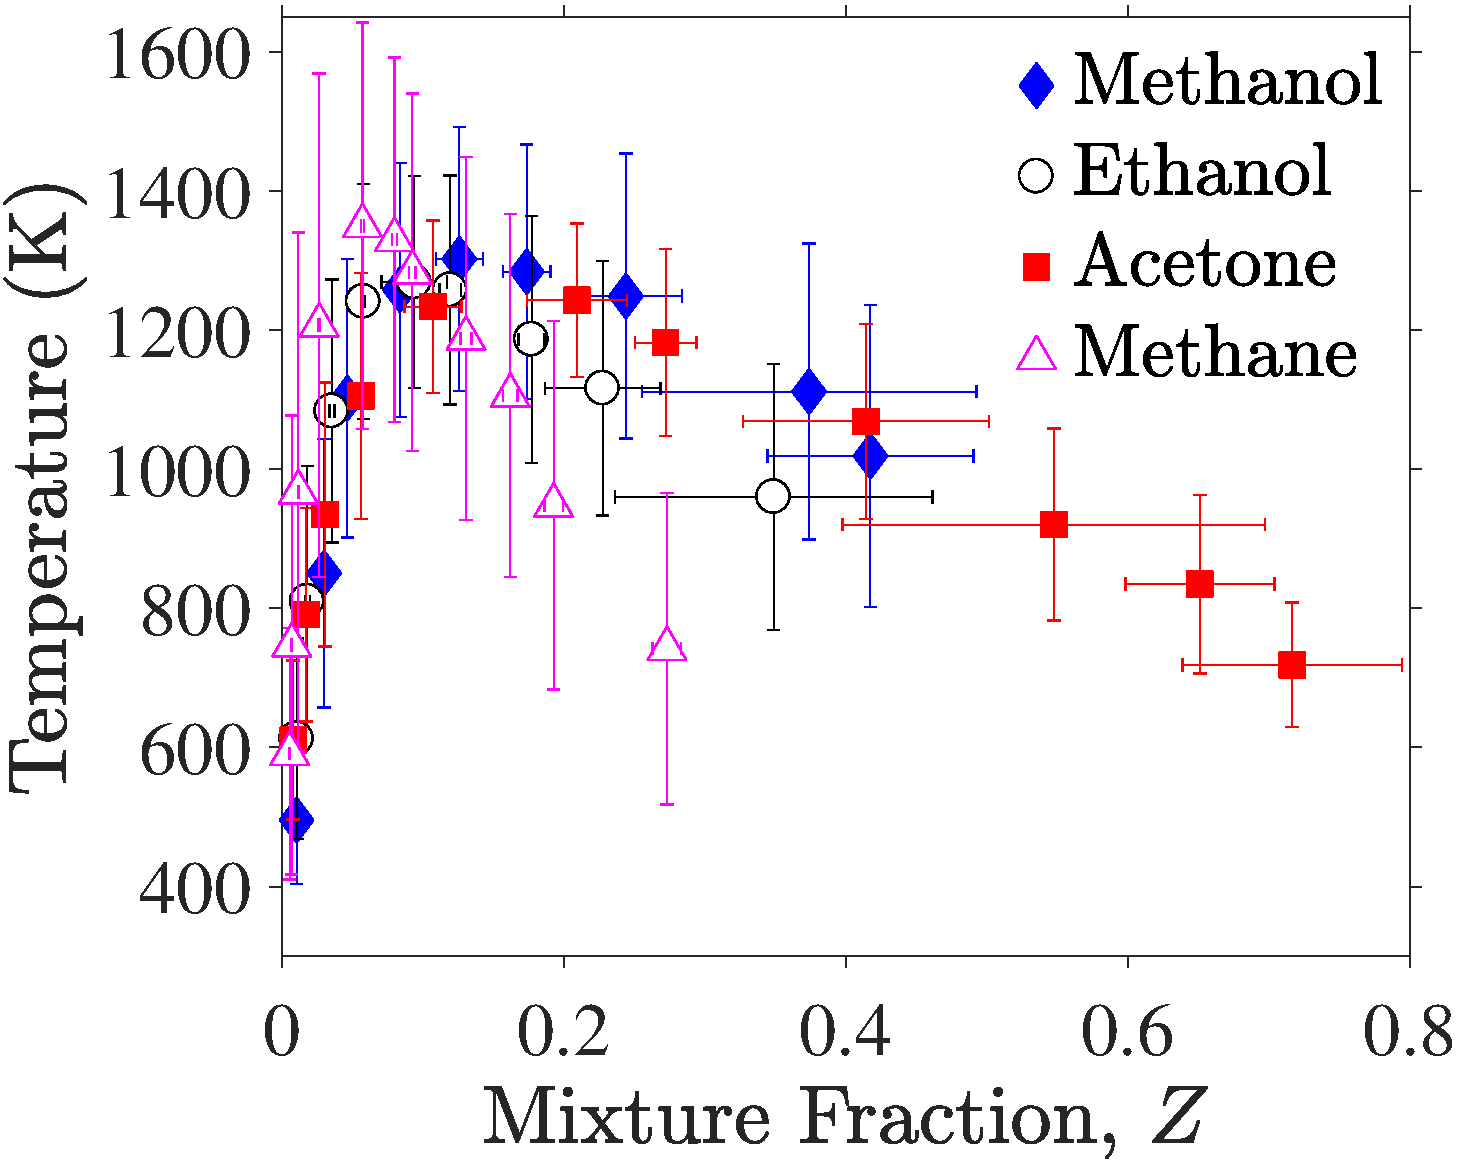
\includegraphics[width=6.7 cm,keepaspectratio]{Temperature_Comparison.pdf}
	\caption[Mean and RMS centerline temperature profiles]{Mean and RMS centerline temperature profiles of methanol, ethanol, acetone, and methane pool fires during their pulsing cycles}
	\label{fig:Temp_Comparison}
\end{figure}
Figure~\ref{fig:Soot_Comparison} shows the soot mass fraction as a function of $z^*$ for the ethanol, acetone, and methane pool fires. No soot was detected within the methanol pool fire. The peak soot mass fraction is achieved at approximately $z^*=0.57~\pm~0.08$. The acetone pool fire has a factor of 5 larger soot mass fraction than ethanol. 
\begin{figure}[h!]
	\centering
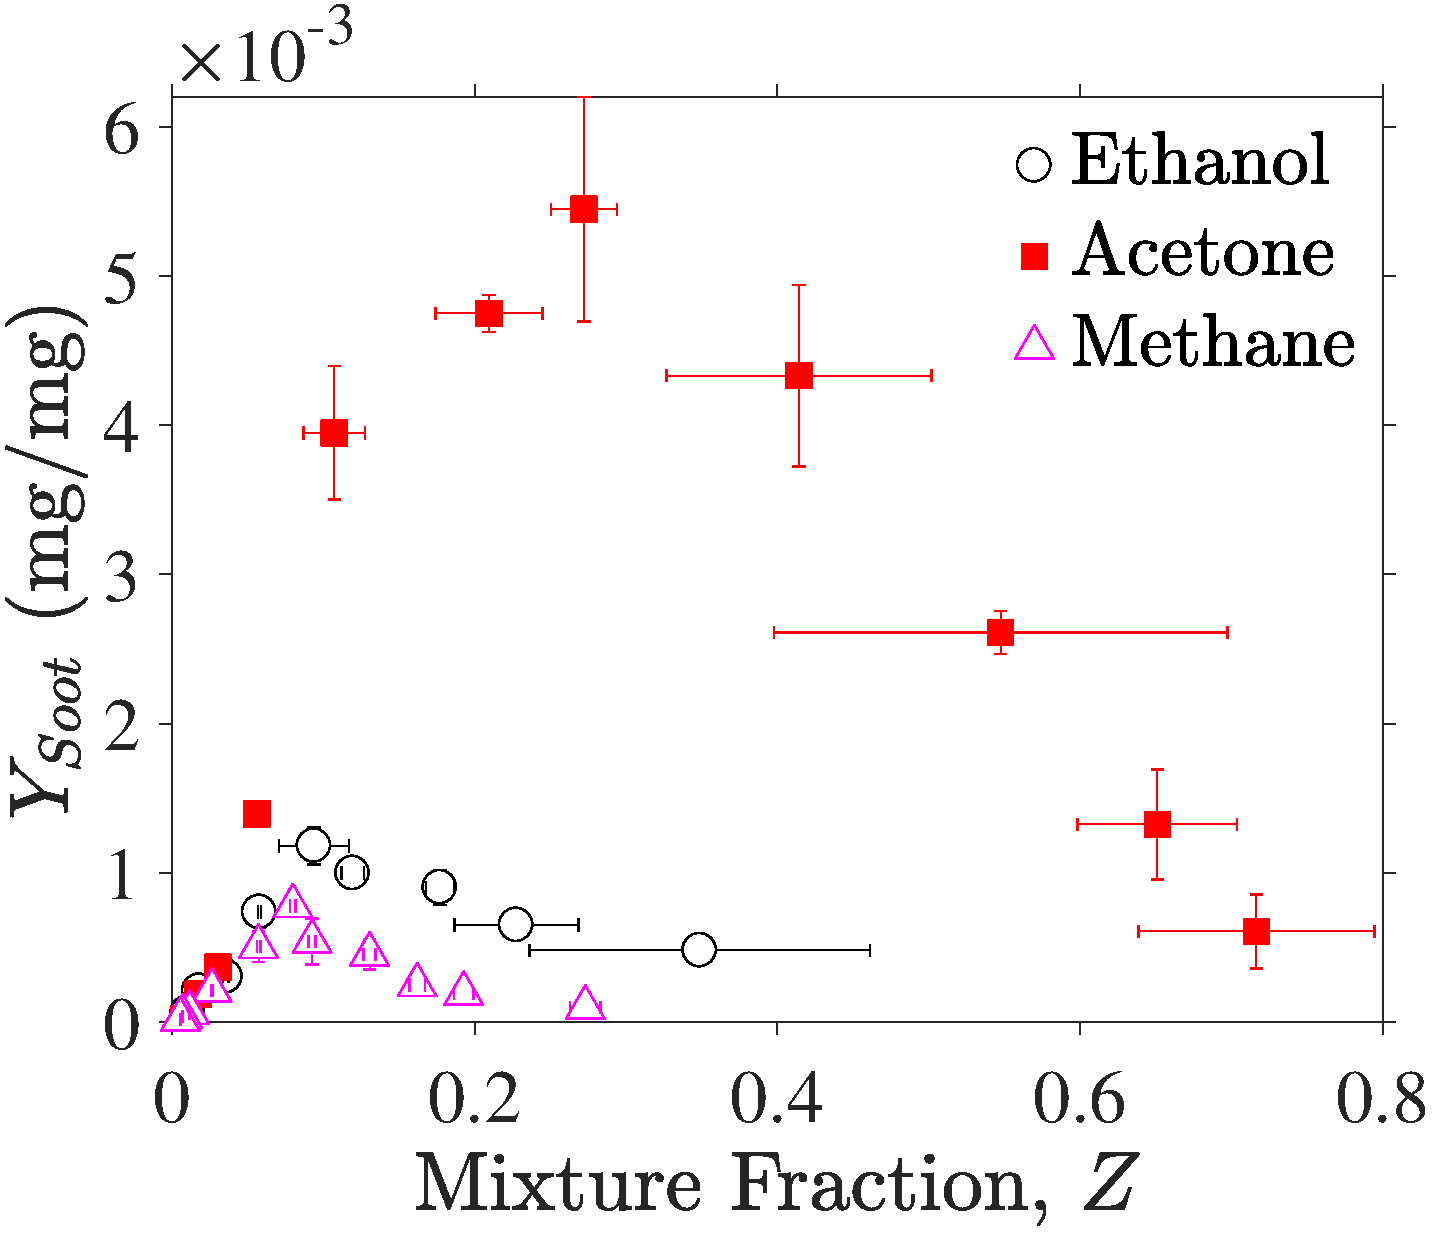
\includegraphics[width=6.7 cm,keepaspectratio]{Soot.pdf}
	\caption[Soot Mass Fraction profiles]{Soot profiles of ethanol, acetone, and methane pool fires}
	\label{fig:Soot_Comparison}
\end{figure}
\subsection{Verifying Gas Species Measurements}
\label{ssec:Verifying_Vol_Frac_Measurements}
The volume fractions of all quantified gaseous species, with uncertainties, is reported in the Supplemental Material (SI). As a way to verify the accuracy of the experimental method, the ratio of carbon to hydrogen atoms contained in all gaseous species is calculated at each vertical measurement location using the following function:
\begin{equation}\label{eq:c2h_ratio}
  \frac{\rm C}{\rm H}=\frac{ \sum  {\rm x}_i \, \bar{X}_{i} }{ \sum {\rm y}_i \, \bar{X}_{i} }
\end{equation}
where the summation is over all measured gaseous species, and ${\rm x}_i$ and ${\rm y}_i$ are the numbers of carbon and hydrogen atoms in the molecule, respectively. The carbon-to-hydrogen ratio of the fuel molecules are reported in Table~\ref{tab:Pool_Fire_Parameters_Table}. As seen in Fig.~\ref{fig:C2H}, the theoretical carbon-to-hydrogen ratio for each fuel, represented by the dotted lines, shows reasonable agreement with the gaseous species.
\begin{figure}[h!]
	\centering
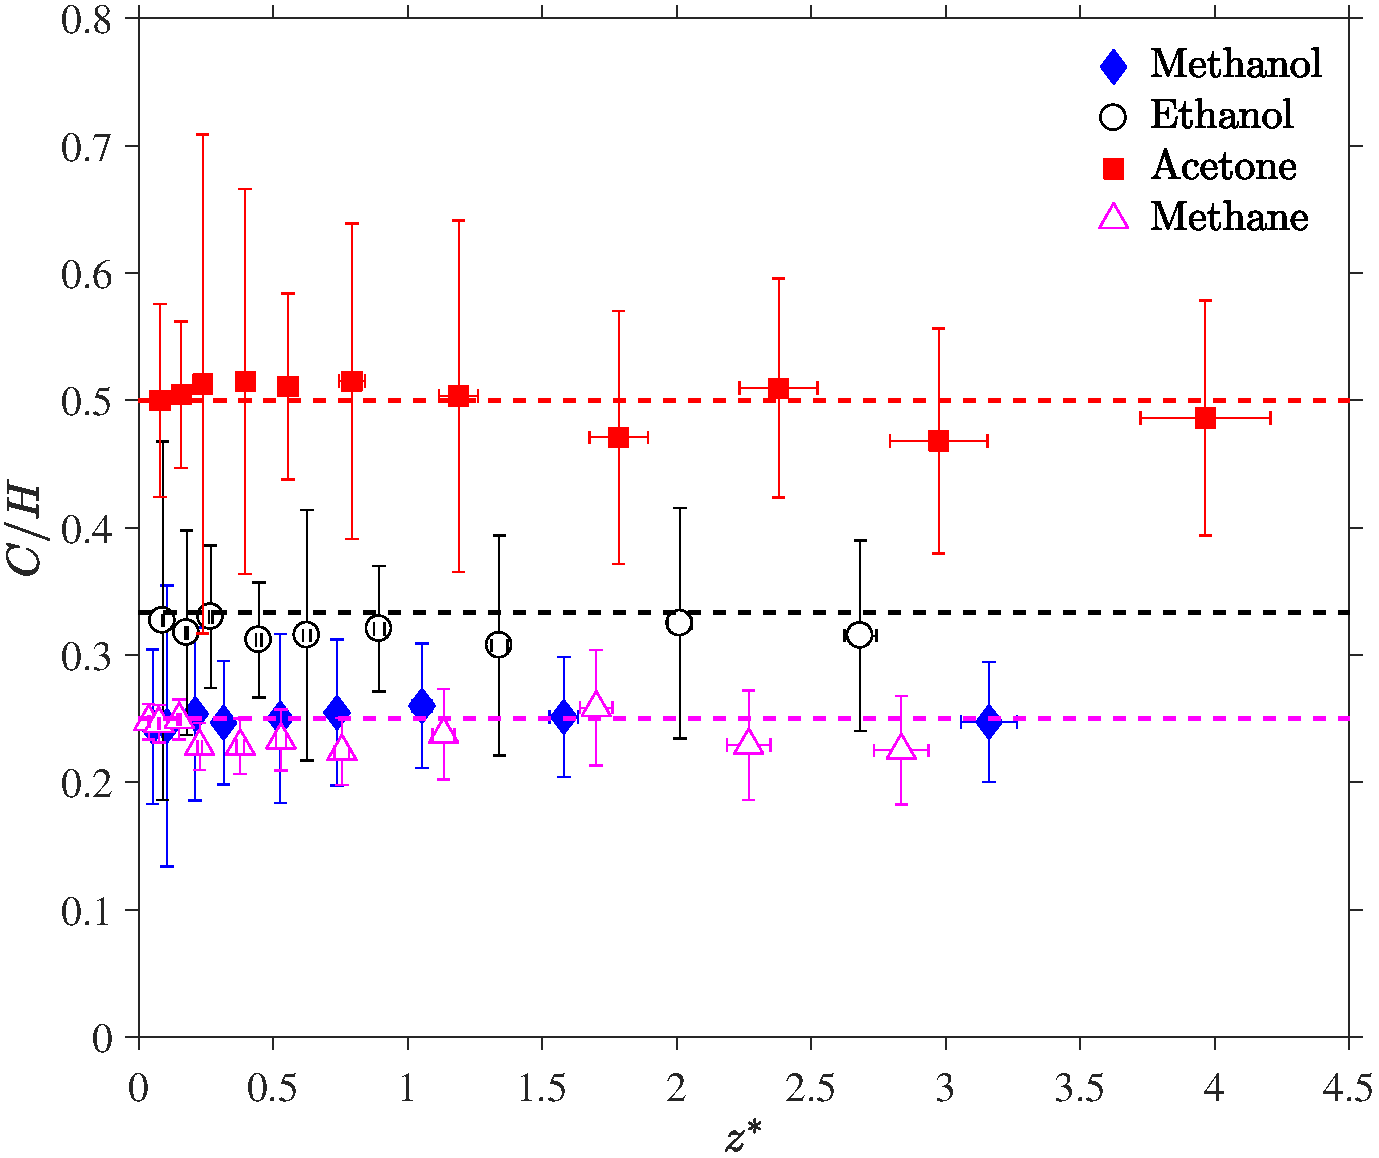
\includegraphics[width=6.7cm, keepaspectratio]{C2H_ratio_Comparison.pdf}
	\caption[Carbon to hydrogen ratio calculated from all species]{Carbon-to-hydrogen ratio calculated from all measured gaseous species compared to the theoretical values.}
	\label{fig:C2H}
\end{figure}

\subsection{Mixture Fraction Analysis}
\label{ssec:Mixture_Faction_Analysis}
Figure~\ref{fig:Mixture_Fraction} shows the mean mass fraction measurements as a function of the mixture fraction for the methanol, ethanol, acetone and methane fires, respectively. The combined expanded uncertainty of each measurement is also presented. The dotted lines represent ideal combustion from Eq.~(\ref{eq:Ideal_rxn}). 
%\begin{figure}[!]
%%	\centering
%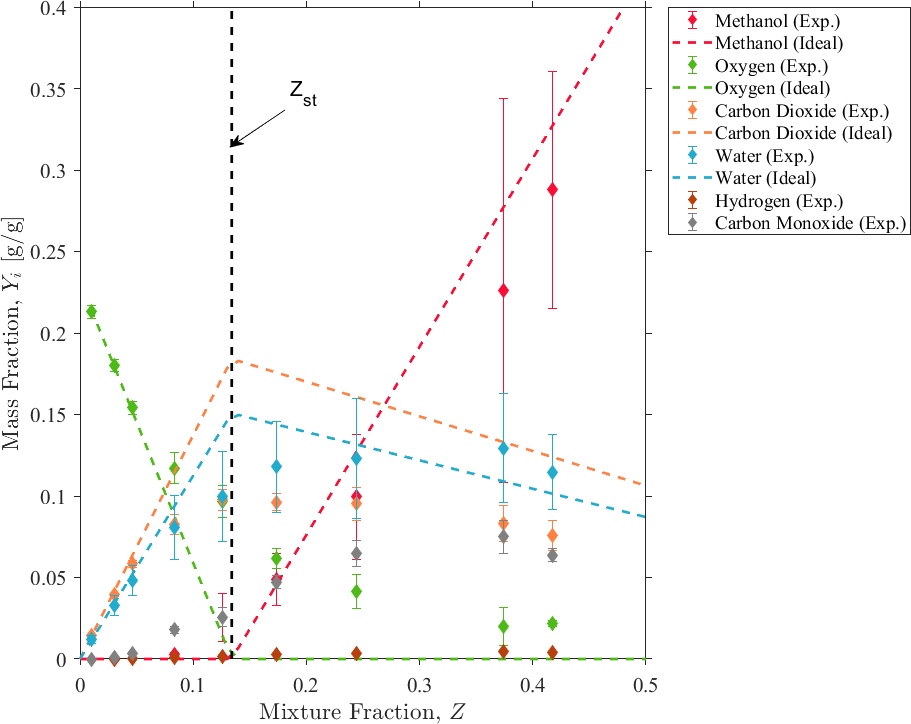
\includegraphics[width=6.7 cm]{Methanol_OVERALL_Mass_Frac_Mix_Frac}
	%\caption[Mean mass fractions as a function of mixture fraction, methanol]{Mean mass fractions as a function of mixture fraction, methanol}
	%\label{fig:Methanol_Mix_Frac}
%\end{figure}
%\begin{figure}[!]
	%\centering
%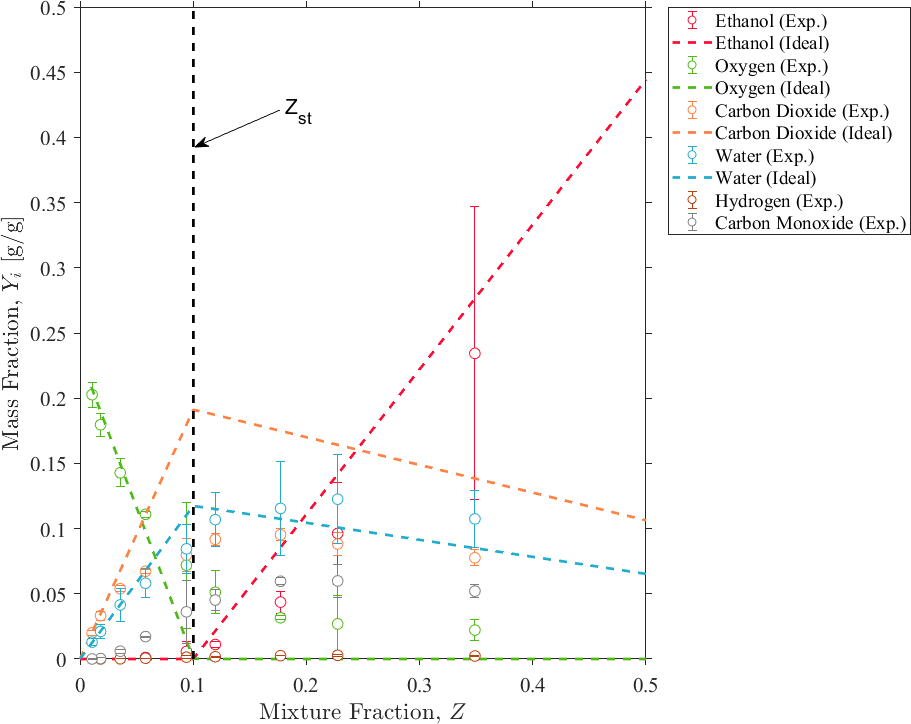
\includegraphics[width=6.7 cm]{Ethanol_OVERALL_Mass_Frac_Mix_Frac}
	%\caption[Mean mass fractions as a function of mixture fraction, ethanol]{Mean mass fractions as a function of mixture fraction, ethanol}
	%\label{fig:Ethanol_Mix_Frac}
%\end{figure}
%\begin{figure}[!]
	%\centering
%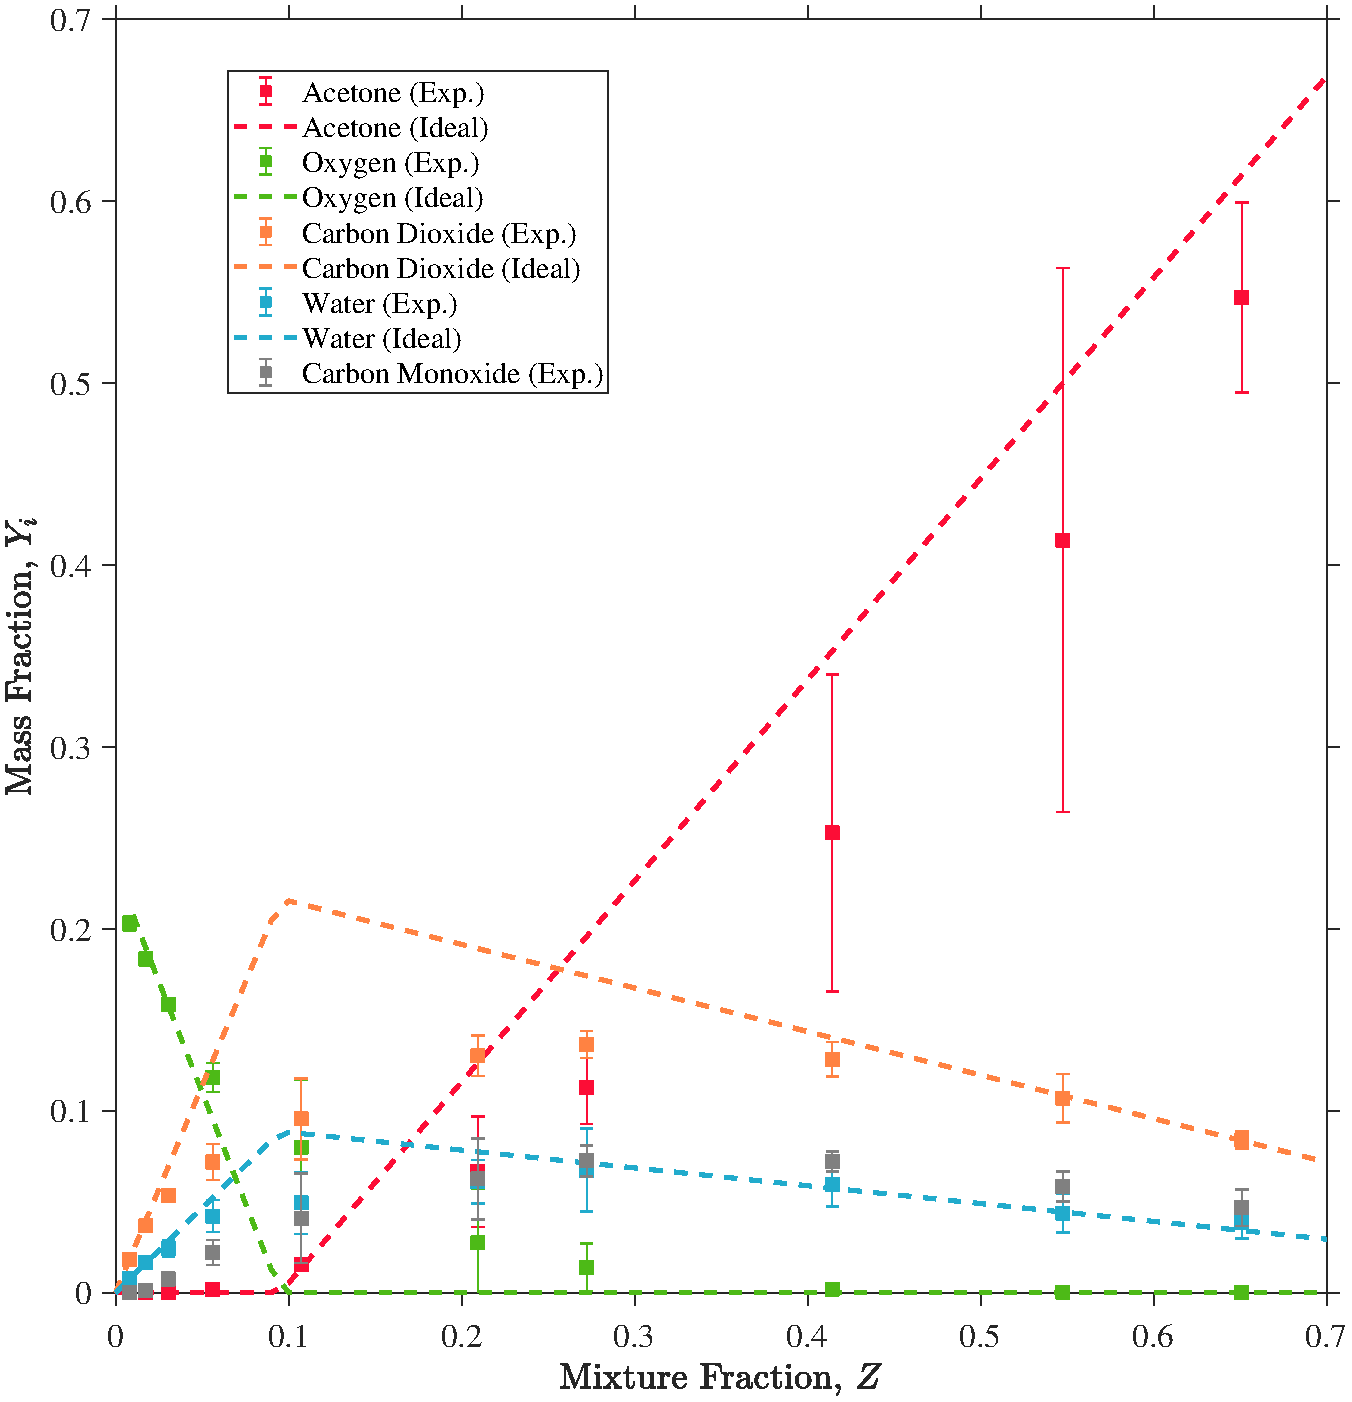
\includegraphics[width=6.7 cm]{Acetone_OVERALL_Mass_Frac_Mix_Frac.pdf}
	%\caption[Mean mass fractions as a function of mixture fraction, acetone]{Mean mass fractions as a function of mixture fraction, acetone}
	%\label{fig:Acetone_Mix_Frac}
%\end{figure}
%\begin{figure}[!]
	%\centering
%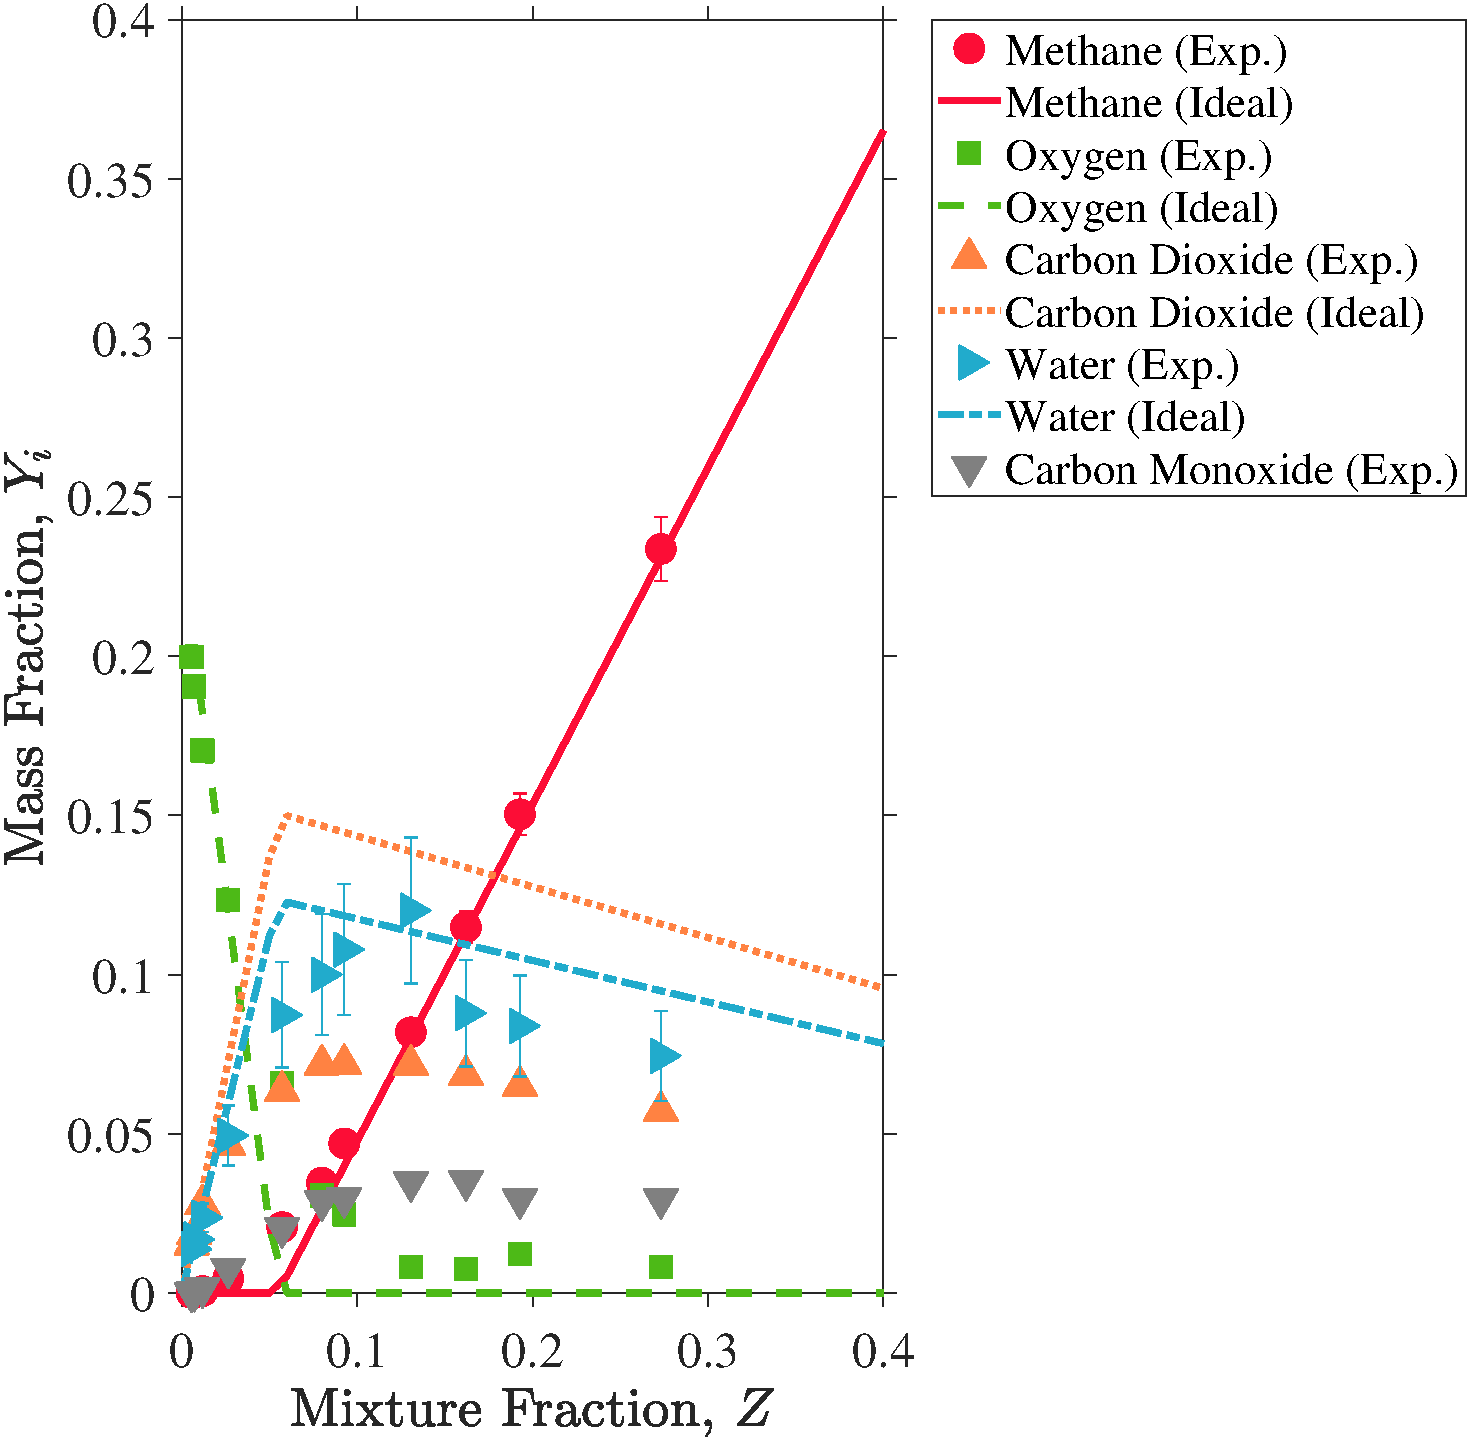
\includegraphics[width=6.7 cm]{Methane_OVERALL_Mass_Frac_Mix_Frac.pdf}
	%\caption[Mean mass fractions as a function of mixture fraction, acetone]{Mean mass fractions as a function of mixture fraction, methane}
	%\label{fig:Methane_Mix_Frac}
%\end{figure}

\begin{figure*}[!t]
	\centering
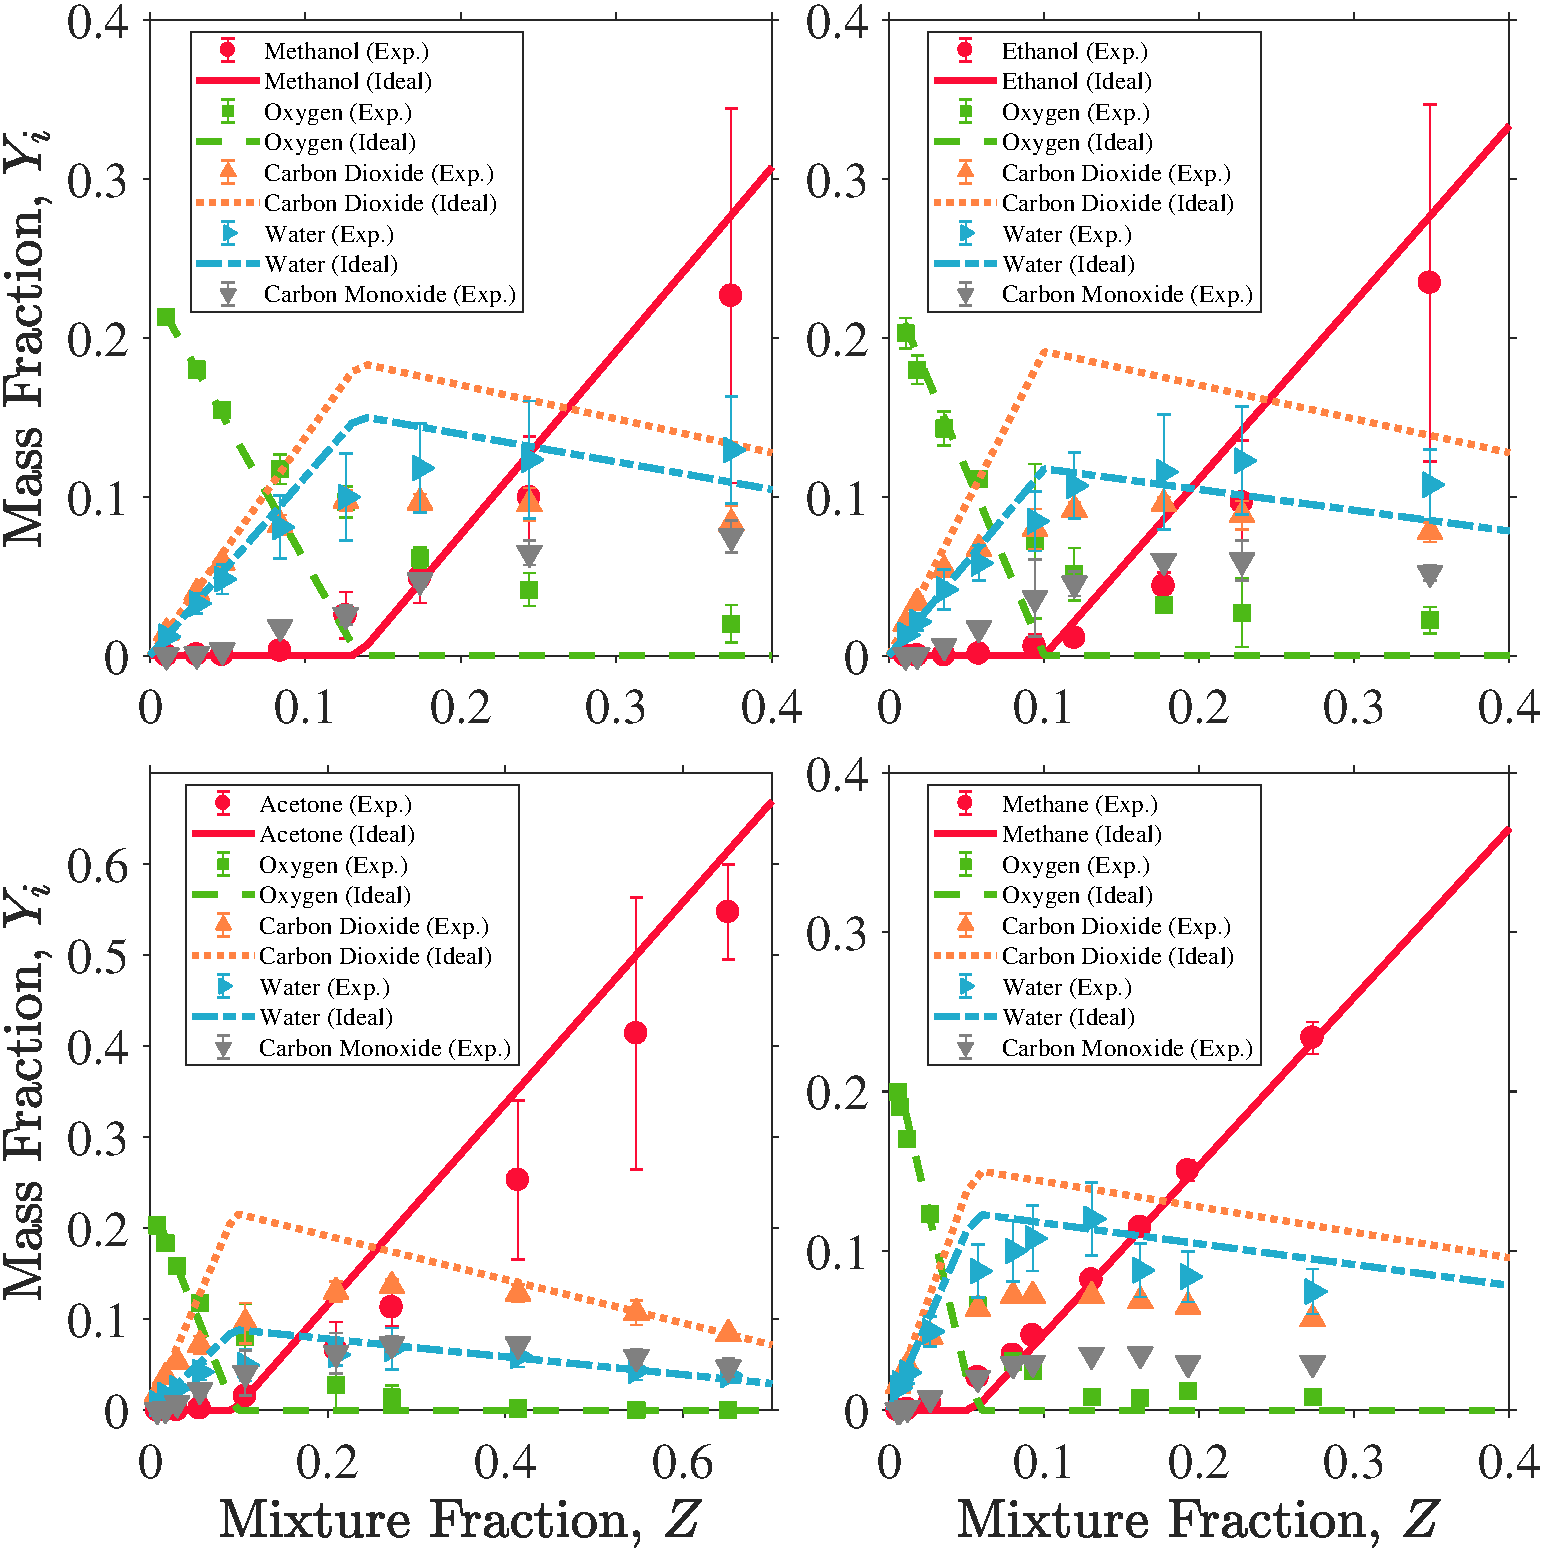
\includegraphics[width=14.27cm,keepaspectratio]{Combined_Mass_Frac_Mix_Frac.pdf}
	\caption[Mean mass fractions as a function of mixture fraction]{Mean mass fractions as a function of mixture fraction for methanol (top left), ethanol (top right), acetone (bottom left), and methane (bottom right) pool fires.}
	\label{fig:Mixture_Fraction}
\end{figure*}

The stoichiometric condition can be identified by the intersection of fuel and oxygen at $Y_i=0$. Where the mixture fraction is much less than stoichiometric, all major gaseous species are in close agreement with the ideal state relations; the measured mass fractions of unburned fuel and $\ch{CO}$ are nearly zero, and the $\ch{O_2}$ is close to its respective theoretical value. The measured mass fraction of $\ch{CO_{2}}$ and $\ch{H_{2}O}$ are found to peak close to the stoichiometric mixture fraction. As the mixture fraction increases, the mass fraction of $\ch{O_2}$ is nearly zero, while the mass fraction of each fuel increases linearly. In the fuel-rich region, the measured mass fraction of $\ch{CO_{2}}$ differs considerably from the ideal state relation due to the substantial portion of $\ch{CO}$ and soot. The over estimation of $\ch{CO_{2}}$ has been observed in other mixture fraction analyses and is attributed to finite rate chemistry effects associated with slow $\ch{CO}$ chemistry~\cite{Sivathanu1990}. For the cases of the liquid pool fires, the over estimation of fuel is likely linked to the presence of other intermediate carbon-containing species close to the fuel surface. This is exemplified in the fuel-rich region for acetone in which the fuel concentration is overestimated while $\ch{CO_{2}}$ is in fair agreement with the hypothetical values; the substantial portion of $\ch{CO}$ and soot, relative to other fuels, could account for the difference. 

\section{Conclusion}
\label{sec:Conclusion}
This study characterizes the structure of several medium-scale pool fires steadily burning in a quiescent environment. Temperature and soot centerline profiles for methanol, ethanol, acetone, and methane is reported. The calculated carbon-to-hydrogen ratio at each location was shown to be in fair agreement with the parent fuel values, which validates the accuracy of the measurements. Major species detected in the centerline profile of the pool fires are represented as a function of mixture fraction. As expected, carbon-containing species are shown to be over-estimated in fuel-rich regions due to the presence of $\ch{CO}$, soot, and other carbon-containing species. 

%% References can be added with or without bibTeX database
%%
%% References with bibTeX database:
%% Note that the PROCI references style is considered Elsevier non-standard.
%% The original Elsevier bibliography style, elsarticle-num.bst prints paper titles as part of the references, which is different from 
\bibliography{References} %%User-specified
\bibliographystyle{elsarticle-num}

%% References without bibTeX database:
%%
 %\begin{thebibliography}{99}
%\bibitem{Westbrook_1984} C. Westbrook, F. Dryer, Progress in Energy and Combustion Science 10 (1984) 1--57.
%\bibitem{Peters_2002} N. Peters, G. Paczko, R. Seiser, K. Seshadri, Combustion and Flame 128 (2002) 38--59.
%\end{thebibliography}

\end{document}

%%
%% End of file `template.tex'.
